%!TeX program = xelatex
\documentclass[12pt,hyperref,a4paper,UTF8]{ctexart}
\usepackage{HDUReport}
\usepackage{listings}
\usepackage{xcolor}

\usepackage{setspace}
\setstretch{1.5} % 设置全局行距为1.5倍

\usepackage{enumitem} % 载入enumitem包以便自定义列表环境
\setlist[itemize]{itemsep=0pt, parsep=0pt} % 设置itemize环境的项目间距和段落间距

\setmainfont{Times New Roman} % 英文正文为Times New Roman


% 自定义 Bash 脚本代码样式
\lstdefinelanguage{bash}{
    keywords={if, else, fi, for, while, do, done, exit, return, local, then, function},
    keywordstyle=\color{blue}\bfseries,
    ndkeywords={echo, printf, cat, grep, awk, sed, tr, chmod, cd, pwd, ls, mv, cp, rm},
    ndkeywordstyle=\color{teal}\bfseries,
    identifierstyle=\color{black},
    sensitive=true,
    comment=[l]{\#},
    commentstyle=\color{gray}\ttfamily,
    stringstyle=\color{red}\ttfamily,
    morestring=[b]",
    morestring=[b]',
}

\lstset{
    language=bash,
    basicstyle=\ttfamily\small, % 设置代码字体和大小
    numbers=left, % 显示行号
    numberstyle=\tiny\color{gray}, % 行号样式
    stepnumber=1, % 行号递增
    numbersep=5pt, % 行号与代码的间距
    backgroundcolor=\color{white}, % 背景颜色
    frame=single, % 代码框样式
    breaklines=true, % 自动换行
    captionpos=b, % 标题位置
    tabsize=4, % Tab 宽度
    showspaces=false, % 不显示空格
    showstringspaces=false, % 不显示字符串中的空格
}

%封面页设置
{   
    %标题
    \title{ 
        \vspace{1cm}
        \heiti \Huge \textbf{Linux系统及应用作业报告} \par
        \vspace{1cm} 
        \heiti \Large {\underline{作业1:Linux操作系统概述}   } 
        \vspace{3cm}
    
    }

    \author{
        \vspace{0.5cm}
        \kaishu\Large 学院\ \dlmu[9cm]{卓越学院} \\ %学院
        \vspace{0.5cm}
        \kaishu\Large 学号\ \dlmu[9cm]{23040447} \\ %班级
        \vspace{0.5cm}
        \kaishu\Large 姓名\ \dlmu[9cm]{陈文轩} \qquad  \\ %学号
        \vspace{0.5cm}
        \kaishu\Large 专业\ \dlmu[9cm]{智能硬件与系统(电子信息工程)} \qquad \\ %姓名 
    }
        
    \date{\today} % 默认为今天的日期,可以注释掉不显示日期
}
%%------------------------document环境开始------------------------%%
\begin{document}

%%-----------------------封面--------------------%%
\cover
\thispagestyle{empty} % 首页不显示页码
%%------------------摘要-------------%%
%\newpage
%\begin{abstract}




%\end{abstract}

%\thispagestyle{empty} % 首页不显示页码

%%--------------------------目录页------------------------%%
% \newpage
% \tableofcontents
% \thispagestyle{empty} % 目录不显示页码

%%------------------------正文页从这里开始-------------------%
\newpage
\setcounter{page}{1} % 让页码从正文开始编号

%%可选择这里也放一个标题
%\begin{center}
%    \title{ \Huge \textbf{{标题}}}
%\end{center}


本次实验选择的 Linux 发行版为 \textbf{Ubuntu 24.04.2 LTS}。

\section{Ubuntu 发行版简介}
Ubuntu 是基于 Debian 的一个开源 Linux 操作系统,首次发布于 2004 年,由英国的 Canonical 公司维护和支持。Ubuntu 以其易用性、稳定性和庞大的社区支持著称,是目前最受欢迎的 Linux 发行版之一。LTS(Long Term Support,长期支持)版本每两年发布一次,提供长达五年的安全更新和维护,适合生产环境和长期使用。

\section{发展过程}
Ubuntu 诞生于 2004 年,旨在为普通用户提供一个易于安装和使用的 Linux 系统。最初的版本基于 Debian,但对桌面环境和驱动支持做了大量优化。随着时间推移,Ubuntu 不断完善,推出了服务器版、云计算版等多个分支,并成为许多云服务和开发环境的首选操作系统。LTS 版本的发布周期和稳定性也使其在企业和教育领域广泛应用。

\section{主要特点}
\begin{itemize}
    \item \textbf{易用性强}:拥有友好的图形界面和丰富的软件中心,适合新手和开发者。
    \item \textbf{社区活跃}:拥有庞大的用户和开发者社区,遇到问题容易获得帮助。
    \item \textbf{软件丰富}:支持 APT 包管理,软件仓库中包含大量常用软件。
    \item \textbf{安全稳定}:LTS 版本提供长期安全更新,适合生产环境。
    \item \textbf{硬件兼容性好}:对主流硬件有良好支持,安装过程简单。
\end{itemize}

\section{适用场景}
Ubuntu 适用于桌面办公、软件开发、服务器部署、云计算、教育科研等多种场景。由于其易用性和稳定性,许多初学者和开发者都选择 Ubuntu 作为入门 Linux 的首选发行版。

\section{选择理由与个人体验}
我选择 Ubuntu 24.04.2 LTS 的原因主要有以下几点:
\begin{itemize}
    \item LTS 版本稳定可靠,适合长期使用。
    \item 社区资源丰富,遇到问题容易查找解决方案。
    \item 软件兼容性好,开发环境搭建方便。
    \item 安装和配置过程简单,适合虚拟机和物理机环境。
\end{itemize}
在实际使用过程中,Ubuntu 的图形界面友好,命令行工具强大,系统运行流畅,能够满足日常学习和开发的需求。

\section{虚拟机软件及安装过程}
本次实验使用的虚拟机软件为 \textbf{VMware Workstation}。在虚拟机中安装 Ubuntu 24.04.2 LTS 的主要步骤如下:

\begin{enumerate}
    \item \textbf{下载 Ubuntu 镜像}:从 Ubuntu 官网下载 24.04.2 LTS 的 ISO 镜像文件。
    \item \textbf{配置虚拟机参数}:设置内存、硬盘大小、CPU 数量等参数。
    \item \textbf{系统初始化}:首次进入系统后,更新软件包并根据需要安装开发工具。
\end{enumerate}

% 可插入关键步骤截图
\begin{figure}[h]
    \centering
    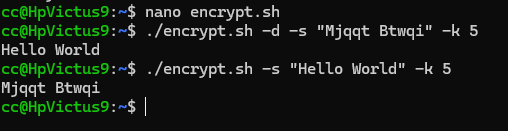
\includegraphics[width=0.9\textwidth]{figures/201.png}
    \caption{WSL使用界面}
\end{figure}





% \begin{figure} % [H] 表示强制当前位置插入
%         \centering
%         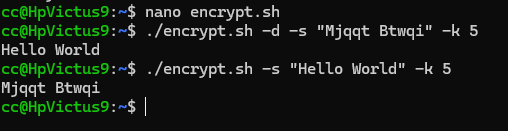
\includegraphics[width=0.9\textwidth]{figures/201.png} % 调整宽度为文本宽度的 80%
%         \caption{WSL指令测试结果} %图片标题
%         \label{fig:example} % 图片标签,用于引用
% \end{figure}


% \begin{figure} % [H] 表示强制当前位置插入
%         \centering
%         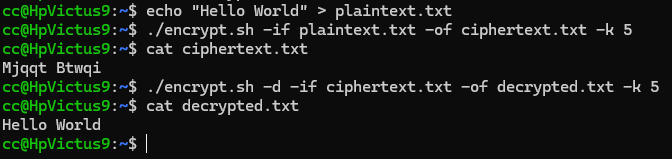
\includegraphics[width=0.9\textwidth]{figures/202.png} % 调整宽度为文本宽度的 80%
%         \caption{WSL文件测试结果} %图片标题
%         \label{fig:example} % 图片标签,用于引用
% \end{figure}


\end{document}